\chapter{User Manual}
Version: 1.0\\\\
Authors: Gianmarco Bacchiorrini 309909, Costabile Di Gregorio 318078, Francesco Gallo
319989\\\\
Legal Disclaimer: The use of jammers is regulated in various jurisdictions and may be
prohibited.\\\\

\section{Introduction}
This jammer was developed in response to the increasing use of microphones and their
potential malicious usage. The device emits high-frequency sound waves capable of creating
interference, preventing the recording of sensitive data that could be exposed to
microphone-based attacks.
In addition, the device is designed to be user friendly and suitable 

\section{Safety Warnings}
\begin{itemize}
    \item The use of jammers is regulated in many countries. It is the user's responsibility observe
    and respect the local laws.
    \item Jammers can interfere with emergency communications and must, therefore, be used
    cautiously.
    \item Avoid prolonged use of the device without supervision.
\end{itemize}

\section{Technical Specifications}
\begin{itemize}
    \item Model: V1.0
    \item Frequencies covered: 22 Khz - 24 Khz
    \item Maximum Operating Power: 100W
    \item Effective Range: The device effectively blocks signals within 30 cm from its position.
    \item Voltage Supply: 12V battery
    \item Battery Life: 13 hours
    \item Rechargeability: No
    \item Wi-Fi: Yes
\end{itemize}

\section{Installation Instructions}
The user will need to connect the Wi-Fi switcher to the system. At this point, the switcher
will enter search mode, looking for the user's phone. Depending on the phone's operating
system, two different procedures can be followed:

[iOS]
\begin{enumerate}
    \item The user accesses the home-iPhone app and, from the dropdown menu, selects to
    connect to the device by clicking on “Add Accessory.” In the figure, “Add Accessory”
    corresponds to the text “Aggiungi accessorio.”
    \begin{figure}[H]
        \centering
        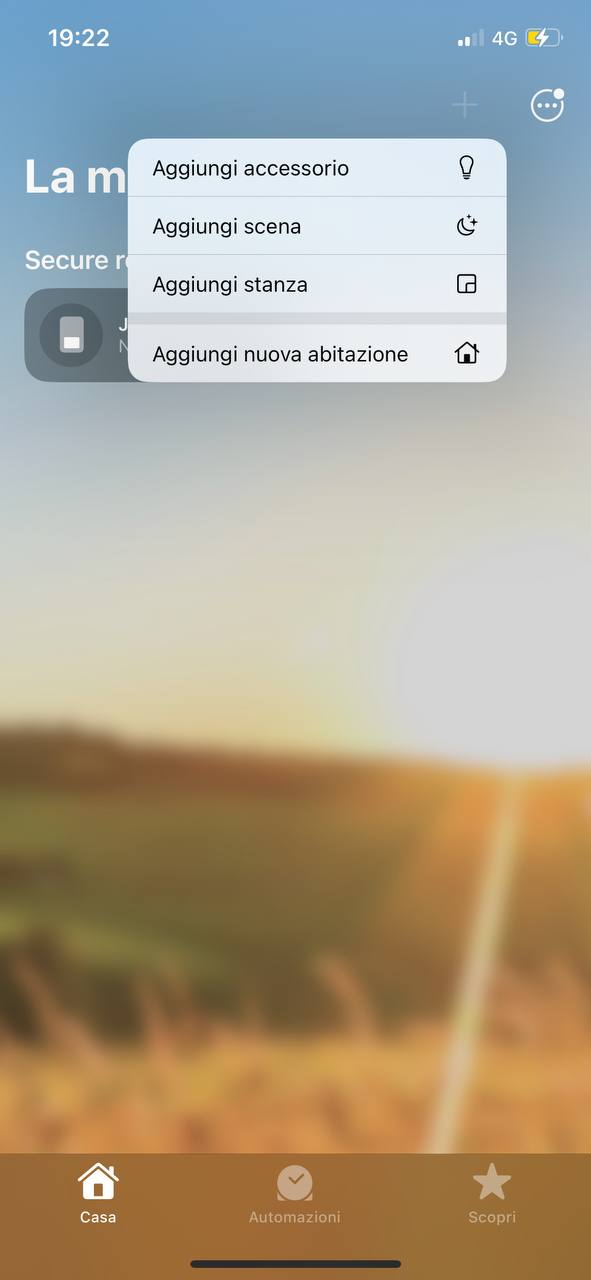
\includegraphics[width=0.3\linewidth]{images/user_manual/1.jpeg}
    \end{figure}
    \item After clicking on "Add Accessory”, the user is able to choose which device to link.
    Please click on “Jammer”
    \begin{figure}[H]
        \centering
        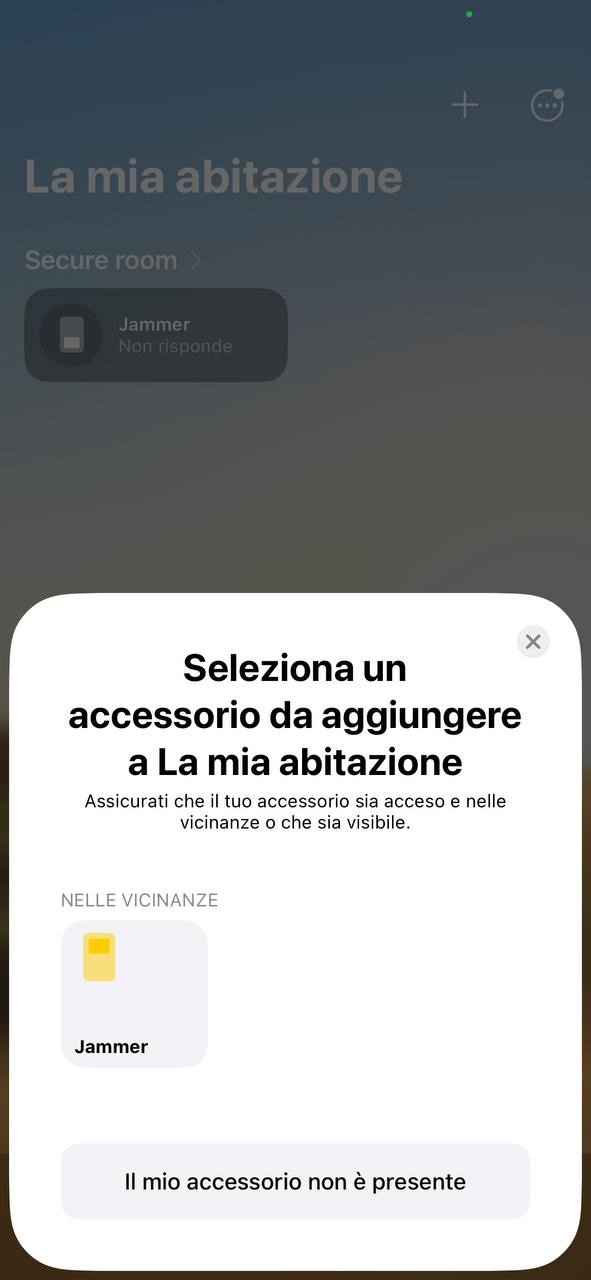
\includegraphics[width=0.3\linewidth]{images/user_manual/2.jpeg}
    \end{figure}
    \item At this point, the user will be prompted for a password that must be entered in the
    designated field.
    Please digit the following password: 12133772 like in the image below.
    \begin{figure}[H]
        \centering
        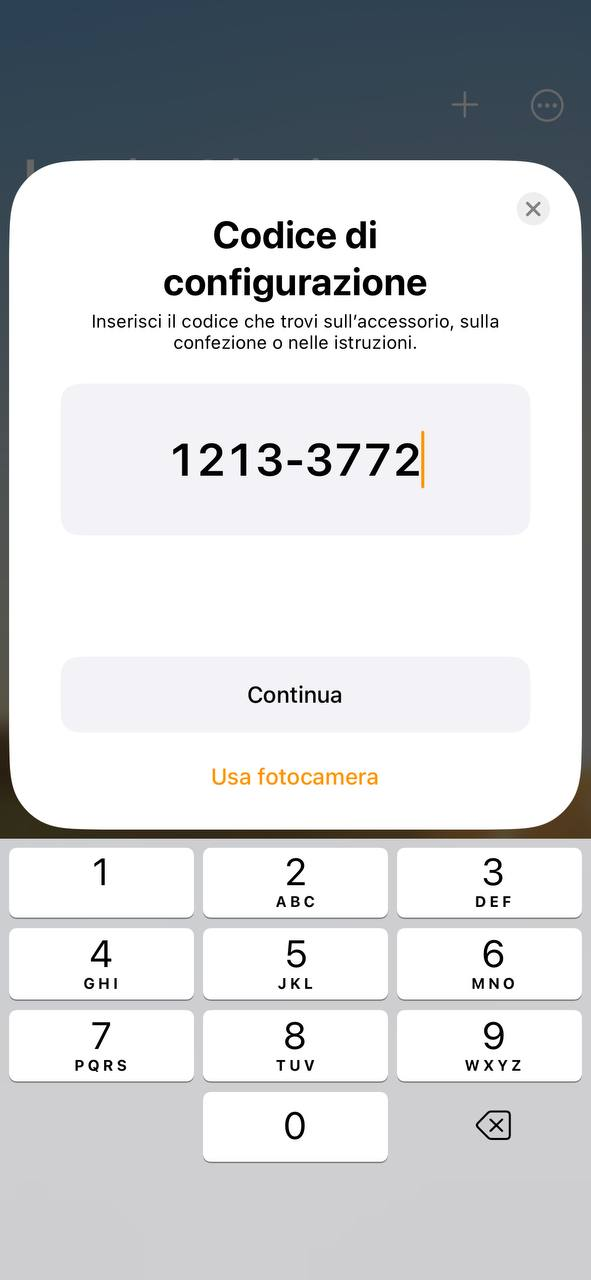
\includegraphics[width=0.3\linewidth]{images/user_manual/3.jpeg}
    \end{figure}
    \item Finally, the user will need to wait for the connection to complete. Afterwards, they
    can use the jammer via the "On" and "Off" commands.
    \begin{figure}[H]
        \centering
        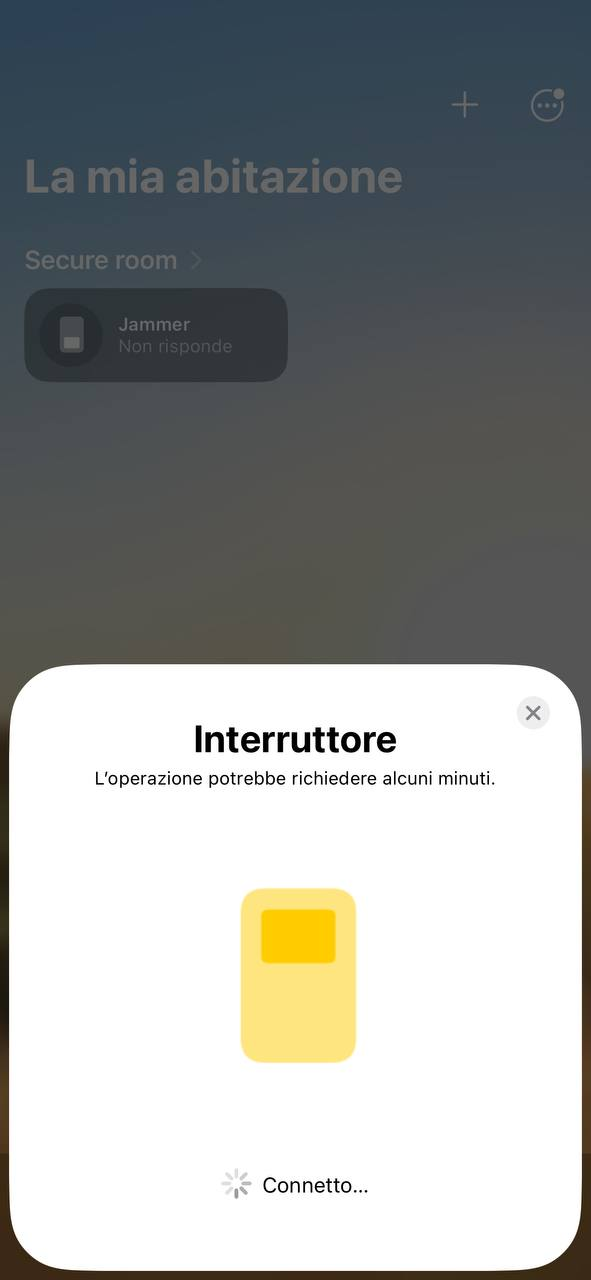
\includegraphics[width=0.3\linewidth]{images/user_manual/4.jpeg}
    \end{figure}
\end{enumerate}

[Others operating system]
\begin{enumerate}
    \item Install any app that supports the protocol. Here are a few suggestions: MQTT.fx
    (Desktop) and MQTT Explorer (Android).
    \item When opening the app, connect to the broker: “broker.hivemq.com” and enter
    “CosFraGia/JammerProject” in the topic field.
    \item Finally, the user will be able to manage the jammer by sending messages that
    contain the payload "Accendi" to activate it and "Spegni" to deactivate it.
\end{enumerate}

\section{Usage Guide}
Once registered with the device’s Wi-Fi, you can remotely turn the jammer on or off.
It is recommended to place the jammer in an open area, near the microphones if you know
them position, so it can function at maximum efficiency.
Since the jammer emits sound waves that prevent unauthorized recordings, be sure to turn
it off once you no longer consider yourself “at risk.”
Prolonged use may cause the device to heat up. In addition, an use without user’s
supervision could cause interference in emergency situations.

\section{Maintenance}
The jammer does not require specific maintenance when not in use.
However, like any electronic device, it should be stored in a dry location, away from water
sources within the home.
It is suggested maintaining the device in a room-temperature location away from heat
sources

\section{Legal Regulations}
The use of jammers is prohibited in certain countries.
It is essential to verify the local laws in the country where the jammer is used, and if
necessary, request a permit from local law enforcement.

\section{Disposal and Recycling}
Follow legal guidelines for the disposal of electronic waste. Generally, do not dispose of the
device with household waste. Instead, locate specific electronic waste disposal areas.
 
